\documentclass[12pt,a4paper,leqno]{report}
\usepackage[utf8]{inputenc}
\usepackage[norsk]{babel}
\usepackage{amsmath}
\usepackage{amsfonts}
\usepackage{amssymb}
\usepackage{graphicx}
\usepackage{float}

\usepackage[left=2cm,right=2cm,top=2cm,bottom=2cm]{geometry}
\author{Krister Borge}
\title{Labrapport \\ \small{prelab}}

\begin{document}
\maketitle
\textbf{Oppgave 1}
\\ Spenningen over en oppladet kondensator med C=1 $\mu$ F
som er koblet til inngangen på et voltmeter halveres på 20 sekunder. Hva er indre resistansen til voltmeteret?

Kondensatoren og voltmeteret skaper denne kretsen:
\begin{figure}[H]
\caption{RC-krets}
\centering
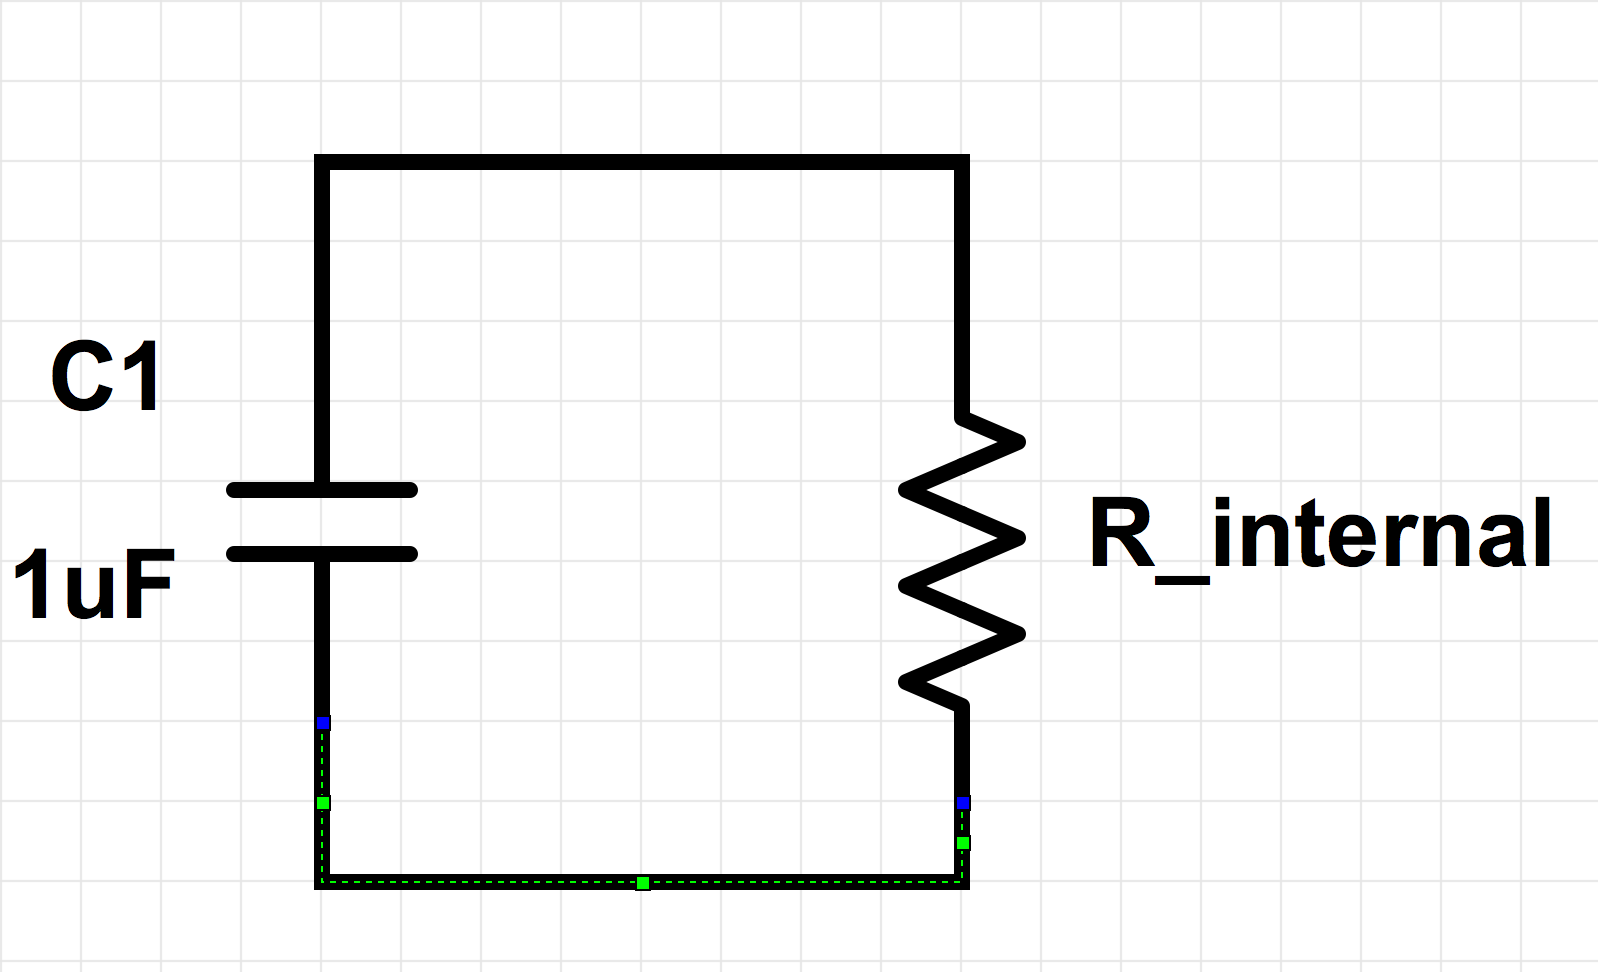
\includegraphics[width=\textwidth]{RC-cirquit.jpg}
\end{figure}
Jeg veit at $\tau=$RC. jeg veit også halveringstiden til kondensatoren som er 20 sekunder. Etter  1 $\tau$  er kondensatoren på 37\% av maks spenning. etter $t=20$ sekunder er spenningen lik $\frac{V_{max}}{2}$.
$$
V(t)=V_0e^{-t/R_{internal}C}
$$

Hvis jeg setter spenningen til 12V blir utrykket:


$$
V(20)=6=12*e^{-20/R_{internal}10^{-6}}
$$
$$
ln(0.5)=ln(e^{-20/R_{internal}10^{-6})}
$$
$$
ln(0.5)=\frac{-20}{R_{internal}10^{-6}}
$$
$$
ln(0.5)=\frac{-20000000}{R_{internal}}
$$
$$
ln(0.5)*R_{internal}=-20000000
$$
$$
R_{internal}=\frac{-20000000}{-0,6931471806}=2.88*10^7=28.8M\Omega
$$
Der $V_0$ er den initielle spenningen i kondensatoren.
Jeg har også at $Q_{max}=CV_{max}$
$F=\frac{Q}{V}$ 

\textbf{Oppgave 2:} 
Lag et MATLAB-skript basert på metodene polyfit og polyval som tilpasser en linje til et sett med datapunkter x,y og viser punktene og den tilpassede linjen på en figur. Dette skriptet kan også brukes i labøvelse 3(Hall-effekt).

\textbf{Oppgave 3:} 
Finn et uttrykk for $B$ dersom vi dreier spolen med konstant vinkelhastighet $\omega$ og måler den maksimale verdien $\epsilon$ for $\epsilon(t)$. Hva er forholdet mellom 
$\omega$ og $t_0-t_1$?
\end{document}